%%%%%%%%%%%%%%%%%%%%%%%%%%%%%%%%%%%%%%%%%
% Short Sectioned Assignment LaTeX Template Version 1.0 (5/5/12)
% This template has been downloaded from: http://www.LaTeXTemplates.com
% Original author:  Frits Wenneker (http://www.howtotex.com)
% License: CC BY-NC-SA 3.0 (http://creativecommons.org/licenses/by-nc-sa/3.0/)
%%%%%%%%%%%%%%%%%%%%%%%%%%%%%%%%%%%%%%%%%

% \documentclass[paper=a4, fontsize=11pt]{scrartcl} % A4 paper and 11pt font size
\documentclass[11pt, a4paper]{book}
\usepackage[T1]{fontenc} % Use 8-bit encoding that has 256 glyphs
\usepackage[utf8]{inputenc}
\usepackage{fourier} % Use the Adobe Utopia font for the document - comment this line to return to the LaTeX default
\usepackage{listings} % para insertar código con formato similar al editor
\usepackage[spanish, es-tabla]{babel} % Selecciona el español para palabras introducidas automáticamente, p.ej. "septiembre" en la fecha y especifica que se use la palabra Tabla en vez de Cuadro
\usepackage{url} % ,href} %para incluir URLs e hipervínculos dentro del texto (aunque hay que instalar href)
\usepackage{graphics,graphicx, float} %para incluir imágenes y colocarlas
\usepackage[gen]{eurosym} %para incluir el símbolo del euro
\usepackage{cite} %para incluir citas del archivo <nombre>.bib
\usepackage{enumerate}
\usepackage{hyperref}
\usepackage{graphicx}
\usepackage{tabularx}
\usepackage{booktabs}

\usepackage[table,xcdraw]{xcolor}
\hypersetup{
	colorlinks=true,	% false: boxed links; true: colored links
	linkcolor=black,	% color of internal links
	urlcolor=cyan		% color of external links
}
\renewcommand{\familydefault}{\sfdefault}
\usepackage{fancyhdr} % Custom headers and footers
\pagestyle{fancyplain} % Makes all pages in the document conform to the custom headers and footers
\fancyhead[L]{} % Empty left header
\fancyhead[C]{} % Empty center header
\fancyhead[R]{Miguel Ángel Posadas Arráez} % My name
\fancyfoot[L]{} % Empty left footer
\fancyfoot[C]{} % Empty center footer
\fancyfoot[R]{\thepage} % Page numbering for right footer
%\renewcommand{\headrulewidth}{0pt} % Remove header underlines
\renewcommand{\footrulewidth}{0pt} % Remove footer underlines
\setlength{\headheight}{13.6pt} % Customize the height of the header

\usepackage{titlesec, blindtext, color}
\definecolor{gray75}{gray}{0.75}
\newcommand{\hsp}{\hspace{20pt}}
\titleformat{\chapter}[hang]{\Huge\bfseries}{\thechapter\hsp\textcolor{gray75}{|}\hsp}{0pt}{\Huge\bfseries}
\setcounter{secnumdepth}{4}
\usepackage[Lenny]{fncychap}

\usepackage{cite} %para incluir citas del archivo <nombre>.bib
\usepackage{apacite}
\hypersetup{%
	citecolor=black
}

% Para las tablas
\usepackage{array}
\usepackage{colortbl}
\usepackage{multirow}
\usepackage{adjustbox}

\usepackage{fancyvrb}
\usepackage{color}

\definecolor{dkgreen}{rgb}{0,0.6,0}
\definecolor{gray}{rgb}{0.5,0.5,0.5}
\definecolor{mauve}{rgb}{0.58,0,0.82}

\newcommand*{\Comment}[1]{\makebox[10cm][l]{#1}}%

\lstset{frame=tb,
  language=Matlab,
  aboveskip=3mm,
  belowskip=3mm,
  showstringspaces=false,
  columns=flexible,
  basicstyle={\small\ttfamily},
  numbers=none,
  numberstyle=\tiny\color{gray},
  keywordstyle=\color{blue},
  commentstyle=\color{dkgreen},
  stringstyle=\color{mauve},
  breaklines=true,
  breakatwhitespace=true,
  tabsize=2,
  numbers=left,
  xleftmargin = 5mm,
  escapechar=\&% char to escape out of listings and back to LaTeX
}


\begin{document}

	% Plantilla portada UGR
	\begin{titlepage}
\newlength{\centeroffset}
\setlength{\centeroffset}{-0.5\oddsidemargin}
\addtolength{\centeroffset}{0.5\evensidemargin}
\thispagestyle{empty}

\noindent\hspace*{\centeroffset}\begin{minipage}{\textwidth}

\centering

\includegraphics[width=0.9\textwidth]{logos/logo_ugr.jpg}\\[1.4cm]

\textsc{ \Large TRABAJO FIN DE GRADO\\[0.2cm]}
\textsc{ GRADO EN INGENIERÍA INFORMÁTICA}\\[1cm]

{\Huge\bfseries Programación eficiente de un algoritmo de procesamiento de la actividad cerebral \\}
\noindent\rule[-1ex]{\textwidth}{3pt}\\[3.5ex]
{\large\bfseries Implementación y optimización mediante paralelización de un algoritmo de análisis fractal de matrices binarias }
\end{minipage}

\vspace{1cm}
\noindent\hspace*{\centeroffset}
\begin{minipage}{\textwidth}
\centering

\textbf{Autor}\\ {Miguel Ángel Posadas Arráez}\\[2.5ex]
\textbf{Director}\\ Juan Ruiz de Miras\\[2cm]

\includegraphics[width=0.3\textwidth]{logos/etsiit_logo.png}\\[0.1cm]
\textsc{Escuela Técnica Superior de Ingenierías Informática y de Telecomunicación}\\
\textsc{---}\\
Granada, Junio de 201x
\end{minipage}
\end{titlepage}


	% Plantilla prefacio UGR
	\thispagestyle{empty}

\begin{center}
{\large\bfseries Programación eficiente de un algoritmo de procesamiento de la actividad cerebral \\ Implementación y optimización mediante paralelización de un algoritmo de análisis fractal de matrices binarias }\\
\end{center}
\begin{center}
Miguel Ángel Posadas Arráez\\
\end{center}

%\vspace{0.7cm}

\vspace{0.5cm}
\noindent{\textbf{Palabras clave}: \textit{Box counting, análisis fractal de matrices binarias, programación paralela, programación GPU}
\vspace{0.7cm}

\noindent{\textbf{Resumen}\\
El procesamiento de datos es una parte esencial en el estudio de diversas enfermedades neurodegenerativas. No obstante, las técnicas actuales para la adquisión de estos datos(resonancia magnética, encefalografía etc...) generan grandes volumenes de datos, lo que conlleva que su procesamiento tenga un gran coste computacional. El propósito de este trabajo es la programación eficiente del método conocido como Box counting para el procesamiento de matrices binarias.  Para la toma de tiempos y con el objetivo de poder hacer diversas comparaciones hemos utilizado dos plataformas con software y hardware diferentes. En un principio, el algoritmo venía programado en Matlab, con el objetivo de obtener una versión más eficiente de este algoritmo implementé una versión secuencial en C++ y posteriormente traté de aprovechar el paralelismo dado por los procesadores multi-core introduciendo la tecnología OpenACC obteniendo aceleraciones de hasta 15.7x. Finalmente, para la obtención de mejores aceleraciones, utilizamos el paradigma de computación de propósito general en unidades de procesamiento gráfico (GPGPU) para aprovechar la arquitectura \textit{Single Instruction, Multiple Data} (SIMD) con el que obtenimos aceleraciones de hasta 77.47x .
	

\cleardoublepage

\begin{center}
	{\large\bfseries Efficient programming of a cerebral processing activity algorithm \\ Implemantation and optimization with parallelization of a binary matrixes fractal analysis algorithm }\\
\end{center}
\begin{center}
	Miguel Ángel Posadas Arráez\\
\end{center}
\vspace{0.5cm}
\noindent{\textbf{Keywords}: \textit{Box counting, Fractal dimension of binary matrix, parallel programming, GPU programming}
\vspace{0.7cm}

\noindent{\textbf{Abstract}\\
Data processing is essential in neurodegenerative diseases studies. However, the existing ways of getting this data (magnetic resonance, electro-encephalography ... ) generate big data volumes, so processing that data has a expensive computing cost. The purpose of this paper is the efficient programming of the Box counting method in order to apply it at binary matrixes processing. They have been used two differents hardware and software platforms to track the time and making comparisons between then. At first, the algorithm was write on Matlab. I \textit{"translated"} that code to C++ with the goal of getting a more efficient sequential algorithm. Then, I tried to parallelize it with OpenACC with the goal of using the multicore CPU and I get a 15.7x speedup. Finally, in order to get the best speedup, I used the general-purpose computing on graphics processing units (GPGPU) to take advantage of the \textit{Single Instruction, Multiple Data} (SIMD) architecture on the graphics processing unit (GPU), getting a speedup of 77.47x.



\cleardoublepage

\thispagestyle{empty}

\noindent\rule[-1ex]{\textwidth}{2pt}\\[4.5ex]

D. \textbf{Juan Ruiz de Miras}, Profesor del Departamento de Lenguajes y Sistemas Informáticos

\vspace{0.5cm}

\textbf{Informo:}

\vspace{0.5cm}

Que el presente trabajo, titulado \textit{\textbf{Programación eficiente de un algoritmo de procesamiento de la actividad cerebral}},
ha sido realizado bajo mi supervisión por \textbf{Miguel Ángel Posadas Arráez}, y autorizo la defensa de dicho trabajo ante el tribunal
que corresponda.

\vspace{0.5cm}

Y para que conste, expiden y firman el presente informe en Granada a Julio de 2021.

\vspace{1cm}

\textbf{El/la director(a)/es: }

\vspace{5cm}

\noindent \textbf{Juan Ruiz de Miras}

\chapter*{Agradecimientos}






	% Índice de contenidos
	\newpage
	\tableofcontents

	% Índice de imágenes y tablas
	\newpage
	\listoffigures

	% Si hay suficientes se incluirá dicho índice
	\listoftables 
	\newpage

	%Si hay suficientes incluir este 
	%\lstlistoflistings

	\chapter{Introducción}


El cálculo de la dimensión fractal de un conjunto de datos es una técnica con una gran multitud de aplicaciones, desde el ámbito económico, -- incluyendo su relación con la premisa del Bitcoin --  {\cite{delfin2016fractal}}, hasta el campo de la medicina y estudio del cuerpo humano, siendo este cálculo útil en la detección de tumores cerebrales {\cite{iftekharuddin2009fractal}}.

La dimensión fractal tiene su cabida en la neurociencia, siendo útil para el procesamiento de la actividad cerebral con el fin de poder estudiar diversas patologías neurodegenerativas \cite{fernandez2001use}. Sin embargo las técnicas actuales para la adquisición de este tipo de datos tales como las electroencefalografías o las resonancias magnéticas, generan grandes volúmenes de datos que implican un alto coste computacional, ya que en función de la dimensión del conjunto de datos, el orden del algoritmo aumenta de manera exponencial, siendo O(n) para conjuntos de datos de una dimensión y O($n^{4}$)  para matrices de cuatro dimensiones.

El propósito de este proyecto es el de la implementación eficiente del algoritmo conocido como Box counting. Para ello, partiendo del algoritmo, inicialmente escrito en el lenguaje de programación Matlab se desarrolla una versión secuencial, escrita en C++ que sirve como base para utilizar diversas tecnologías,como OpenACC y CUDA, con el fin de aprovechar el paralelismo que proporcionan los microprocesadores actuales así como la arquitectura SIMD (\textit{Single Instruction Multiple Data}) presente en las tarjetas gráficas.

	
	\chapter{Plan de proyecto}

En este apartado se presenta la planificación seguida a lo largo de todo el proyecto. Se especifican una serie de tareas diferenciadas entre sí que a continuación serán detalladas en profundidad.\\ Para dar por finalizada una tarea, y así poder pasar a la siguiente, ésta ha debido ser revisada previamente por el tutor. \\ Dentro del plan de estudios de la titulación, el trabajo de fin de grado tiene una carga de 12 créditos ECTS, y teniendo en cuenta que cada crédito ECTS equivale a 25 horas obtenemos, que el proyecto debe ser completado en 300 horas. De esta manera la planificación que procederemos a desarrollar en esta sección, se elabora considerando que el horario va a ser de lunes a viernes con jornadas de 3 horas de trabajo.\\

\section{Descripción de las tareas}
\subsection{Planificación del proyecto}
\label{tareaPlanificacion}
La planificación del proyecto corresponde a la primera tarea. Se subdivide el proyecto en las propias tareas que se están comentando en este punto, se realiza una estimación de tiempo de la que se genera un diagrama de Gantt que se puede consultar en la Figura \ref{fig:Gantt}, y una estimación de costos, que queda reflejada en la sección \ref{Costos}.\\

Se estima que esta tarea tendrá una duración de 5 horas.

\subsection{Estudio del algoritmo Box counting}
Con esta tarea se deja un tiempo para obtener formación sobre el algoritmo Box counting, conocer cómo funciona el \textit{"Fixed grid scan"}, y entender la implementación inicial escrita en Matlab. Para la realización de esta tarea se requiere de la adquisición de unas nociones básicas de Matlab debido al desconocimiento previo del lenguaje.\\

Se estima que esta tarea tendrá una duración de 10 horas.

\subsection{Implementación en C++ del algoritmo Box counting}
Una vez se haya comprendido el funcionamiento del algoritmo con el que se va a trabajar a lo largo de todo el proyecto, se procederá a su implementación secuencial en C++. Dentro de esta tarea, entra la comprobación de la corrección del código implementado, comprobando que es válido y funciona correctamente con datos reales de activación cerebral.\\

Se estima que esta tarea tendrá una duración de 10 horas.

\subsection{Experimentación y toma de tiempos del algoritmo sin paralelizar}
Se deja como tarea una etapa para la experimentación y toma de tiempos del algoritmo secuencial obtenido de la tarea anterior. Para la toma de tiempos se seguirá la metodología que se expone en el capítulo siguiente. El objetivo de la toma de tiempos del algoritmo secuencial es poder realizar comparaciones con las versiones que se implementen posteriormente, y medir que versión proporciona mejores aceleraciones.\\

Se estima que esta tarea tendrá una duración de 5 horas.

\subsection{Paralelización del algoritmo con OpenACC}
Se planifica una tarea que conlleva la búsqueda de bibliografía y el estudio del estándar de programación OpenACC. El objetivo de esto es poder añadir al código secuencial las directivas OpenACC necesarias para explotar el paralelismo que nos aporta el uso de una CPU multicore.\\

Se estima que esta tarea tendrá una duración de 70 horas.

\subsection{Experimentación y toma de tiempos de la paralelización con OpenACC}
Se planifica como tarea una etapa para la experimentación y toma de tiempos del código resultante de la tarea anterior. Además se analizarán los tiempos obtenidos y se compararán con los tiempos obtenidos en la etapa de experimentación del código secuencial mediante el cálculo de las aceleraciones.\\

Se estima que esta tarea tendrá una duración de 10 horas.

\subsection{Paralelización del algoritmo con CUDA}
Se planifica una tarea que conlleva la búsqueda de bibliografía y el estudio de la plataforma de programación CUDA. De esta manera, en esta fase del proyecto, se implementará todo lo necesario para aprovechar la computación de propósito general en unidades de procesamiento gráfico (GPGPU) para aprovechar las tarjetas gráficas de la compañía Nvidia.\\

La paralelización con CUDA es un poco más compleja que la paralelización con OpenACC, por tanto, para realizar esta tarea se empezará implementado la versión en 2D, y partiendo de esa versión como base, se desarrollarán la versión 3D y 4D.\\

Se estima que esta tarea tendrá una duración de 110 horas.

\subsection{Experimentación y toma de tiempos de la paralelización con CUDA}
Se deja como tarea una etapa para la experimentación y toma de tiempos del código resultante de la tarea anterior. Además se analizarán los tiempos obtenidos y se compararán con los tiempos obtenidos en la etapa de experimentación del código secuencial y con la etapa de experimentación del código paralelizado con OpenACC mediante el cálculo de las aceleraciones.\\

Se estima que esta tarea tendrá una duración de 20 horas.

\subsection{Análisis de los resultados obtenidos}
El objetivo de esta tarea, es dejar un tiempo para la comparación de todos los resultados obtenidos en las etapas de experimentación y toma de tiempos, así como discusión y redacción de conclusiones sobre los resultados obtenidos.\\

Se estima que esta tarea tendrá una duración de 20 horas.

\subsection{Elaboración de la memoria}
Durante el desarrollo de todo el proyecto se irá elaborando una memoria a modo de documentación del trabajo realizado, aunque se estiman 30 horas adicionales para terminarla.

\subsection{Preparación de la defensa ante el tribunal}
Tras la entrega del trabajo, se deja un tiempo para la elaboración del material necesario para la defensa y exposición del proyecto ante el tribubal.\\

Se estima que esta tarea tendrá una duración de 10 horas.


\section{Diagrama de Gantt}
Como anticipábamos en \textit{"\nameref{tareaPlanificacion}"}, la primera etapa del proyecto es la planificación temporal del mismo. Para ello el primer paso es la división del proyecto en tareas y su correspondiente especificación. A continuación, se realiza una estimación de los días necesarios que tomará cada tarea, teniendo en cuenta que se trabajará en jornadas de 3 horas diarias de lunes a viernes. Finalmente, se hace una planificación temporal de todas las tareas en base a la estimación de tiempo realizada, obteniendo así el diagrama de la Figura \ref{fig:Gantt}. En la tabla \ref{fig:Planificacion} se puede consultar la estimación de cada tarea así como, su fecha de inicio y finalización\\ Debido a la falta de experiencia en un proyecto de este tipo, esta especificación puede que no sea suficientemente detallada, en los siguientes capítulos se profundizará más en la descripción de las distintas tareas.\\ Esto es una planificación inicial del proyecto, como en todo proyecto es posible que surjan inconvenientes que retrasen alguna de las tareas o que se hayan subestimado alguna de ellas.
\newpage
\begin{figure}[h]
    \raggedright
    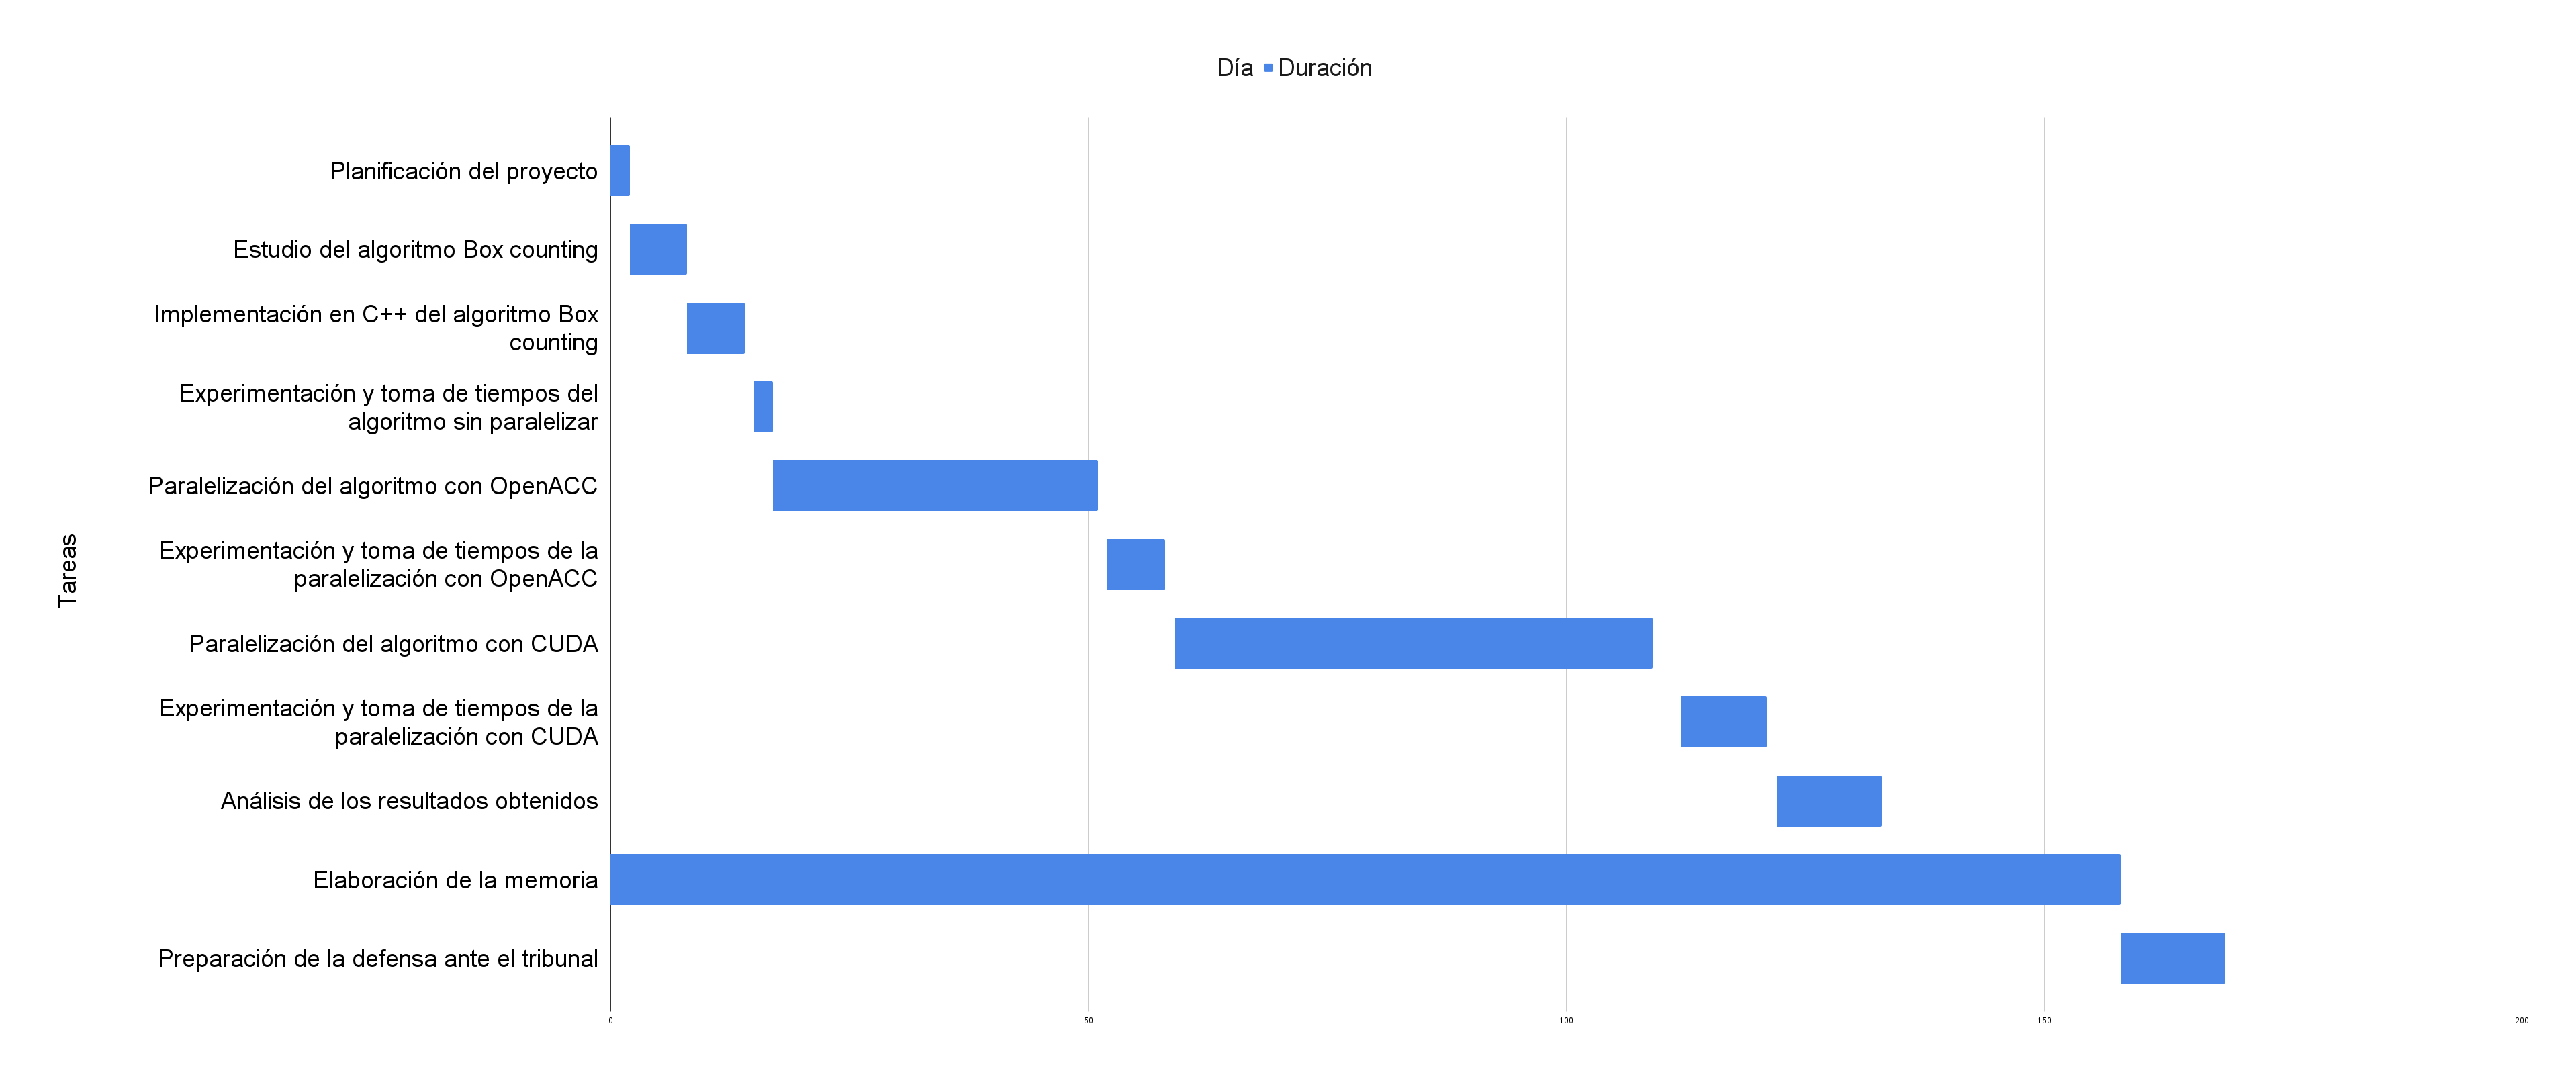
\includegraphics[scale=0.145]{img/Diagrama de Gantt2.png}
    \caption{Diagrama de Gantt}
    \label{fig:Gantt}
\end{figure}

\begin{table}[H]
    \centering
    \begin{adjustbox}{max height=\textheight, max width=\textwidth}
    \begin{tabular}{|clllrrl|} 
    \hline
    \rowcolor{black} \multicolumn{1}{|l}{}  & \textcolor{white}{Tareas} & \textcolor{white}{Fecha de inicio}         & \textcolor{white}{Fecha de finalización} & \textcolor{white}{Horas estimadas}&\\                                      
    \hline
    \rowcolor{white} \multicolumn{1}{|l}{}  & \textcolor{black}{Planificación del proyecto} & \textcolor{black}{1/2/2021}         & \textcolor{black}{3/2/2021} & \textcolor{black}{5}&\\
    \hline
    \rowcolor{white} \multicolumn{1}{|l}{}  & \textcolor{black}{Estudio del algoritmo Box counting} & \textcolor{black}{3/2/2021}         & \textcolor{black}{9/2/2021} & \textcolor{black}{10}&\\  
    \hline
    \rowcolor{white} \multicolumn{1}{|l}{}  & \textcolor{black}{Implementación en C++ del algoritmo Box counting} & \textcolor{black}{9/2/2021}         & \textcolor{black}{15/2/2021} & \textcolor{black}{10}\\
    \hline
    \rowcolor{white} \multicolumn{1}{|l}{}  & \textcolor{black}{Experimentación y toma de tiempos del algoritmo sin paralelizar} & \textcolor{black}{16/2/2021}         & \textcolor{black}{18/2/2021} &\textcolor{black}{5}&\\
    \hline
    \rowcolor{white} \multicolumn{1}{|l}{}  & \textcolor{black}{Paralelización del algoritmo con OpenACC} & \textcolor{black}{18/2/2021}         & \textcolor{black}{24/3/2021} &\textcolor{black}{70}\\
    \hline
    \rowcolor{white} \multicolumn{1}{|l}{}  & \textcolor{black}{Experimentación y toma de tiempos de la paralelización con OpenACC} & \textcolor{black}{25/3/2021}         & \textcolor{black}{31/3/2021} &\textcolor{black}{10}\\
    \hline
    \rowcolor{white} \multicolumn{1}{|l}{}  & \textcolor{black}{Paralelización del algoritmo con CUDA} & \textcolor{black}{1/4/2021}         & \textcolor{black}{21/5/2021} &\textcolor{black}{110}\\
    \hline
    \rowcolor{white} \multicolumn{1}{|l}{}  & \textcolor{black}{Experimentación y toma de tiempos de la paralelización con CUDA} & \textcolor{black}{24/5/2021}         & \textcolor{black}{2/6/2021} &\textcolor{black}{20}\\
    \hline
    \rowcolor{white} \multicolumn{1}{|l}{}  & \textcolor{black}{Análisis de los resultados obtenidos} & \textcolor{black}{3/6/2021}         & \textcolor{black}{14/6/2021} &\textcolor{black}{20}&\\
    \hline
    \rowcolor{white} \multicolumn{1}{|l}{}  & \textcolor{black}{Elaboración de la memoria} & \textcolor{black}{1/2/2021}         & \textcolor{black}{9/7/2021} &\textcolor{black}{30}&\\
    \hline
    \rowcolor{white} \multicolumn{1}{|l}{}  & \textcolor{black}{Preparación de la defensa ante el tribubal} & \textcolor{black}{9/7/2021}         & \textcolor{black}{20/7/2021} &\textcolor{black}{10}&\\                                  
    \hline
    \end{tabular}
    \end{adjustbox}
    \caption{Planificación temporal de las tareas}
    \label{fig:Planificacion}
\end{table}

\section{Recursos}
\subsection{Recursos Humanos}
Para la realización del proyecto se cuenta con Miguel Ángel Posadas Arráez como autor del mismo, y con el Profesor Dr. Juan Ruiz de Miras como tutor encargado de la supervisión del mismo.

\subsection{Recursos Software}
\label{RecursosSoftware}
Debido a que este proyecto corresponde al ámbito académico, se presta especial atención en utilizar herramientas con licencia libre, o que sean accesibles mediante la adquisición de algún tipo de licencia de estudiante, beneficiandonos así, de las ventajas que nos proporciona pertenecer a la Universidad de Granada.\\

\begin{itemize}
    \item Como alternativa a Matlab, se utiliza Octave. \cite{unknown-author-2021B}.
    \item Como herramienta de control de versiones, se utiliza GitHub, siendo posible obtener una licencia de estudiante en la siguiente referencia \cite{unknown-author-2021}.
    \item Para la elaboración de hojas de cálculo y generación de gráficos, se utiliza la suite ofimática de Google, accediendo siempre con la cuenta corporativa de la Universidad de Granada (dominio go.ugr.es).
    \item Para la elaboración de la memoria LaTeX como procesador de textos. \cite{unknown-author-no-dateD}.
    \item Para la paralelización mediante el uso de tarjeta gráfica, se utiliza el CUDA Toolkit, \cite{unknown-author-no-date}.
    \item Para la paralelización mediante el uso de los mútliples núcleos de la CPU, se utiliza OpenACC. \cite{unknown-author-no-dateB}.
    \item El sistema operativo del equipo principal utilizado para el desarrollo del proyecto es Ubuntu 20.04.2 LTS. \cite{unknown-author-no-dateE}.
\end{itemize}

\subsection{Recursos Hardware}
\label{RecursosHardware}
Para el desarrollo del proyecto se utilizan dos equipos, un ordenador portatil y un servidor. En la tabla \ref{fig:Hardware} quedan reflejadas las características más importantes de los distintos equipos.

\begin{table}[H]
    \centering
    \begin{adjustbox}{max height=\textheight,max width=\textwidth}
    \begin{tabular}{|clllrrl|} 
    \hline
    \rowcolor{black} \multicolumn{1}{|l}{}   & \textcolor{white}{Plataforma}         & \textcolor{white}{} \\  
    \hline
    \rowcolor{white} \multicolumn{1}{|l}{Plataforma}   & \textcolor{black}{PC}         & \textcolor{black}{Servidor} \\  
    \hline
    \rowcolor{white} \multicolumn{1}{|l}{Sistema Operativo}    & \textcolor{black}{Ubuntu 20.04 LTS $x86-64$}         & \textcolor{black}{Debian Linux 5.8.10-1 $x86-64$}        \\                                                            
    \hline
    \midrule
    \hline
    \rowcolor{black} \multicolumn{1}{|l}{}   & \textcolor{white}{CPU}         & \textcolor{white}{} \\  
    \hline
    \rowcolor{white} \multicolumn{1}{|l}{Model}    & \textcolor{black}{Intel(R) Core(TM) i7-7700HQ CPU @ 2.80GHz}         & \textcolor{black}{2 x Intel(R) Xeon(R) Silver 4210 CPU @ 2.20GHz}        \\ 
    \hline
    \rowcolor{white} \multicolumn{1}{|l}{Cores-thread}    & \textcolor{black}{4-8}         & \textcolor{black}{20-40}        \\  
    \hline
    \rowcolor{white} \multicolumn{1}{|l}{RAM}    & \textcolor{black}{12 GB}         & \textcolor{black}{96 GB}        \\ 
    \hline
    \rowcolor{black} \multicolumn{1}{|l}{}   & \textcolor{white}{GPU}         & \textcolor{white}{} \\  
    \hline                          
    \rowcolor{white} \multicolumn{1}{|l}{Model}    & \textcolor{black}{GeForce GTX 1050 Mobile}         & \textcolor{black}{GeForce RTX 3090}        \\ 
    \hline
    \rowcolor{white} \multicolumn{1}{|l}{Computing Capability}   & \textcolor{black}{6.1}         & \textcolor{black}{8.0} \\  
    \hline
    \rowcolor{white} \multicolumn{1}{|l}{Arquitectura}   & \textcolor{black}{Pascal}         & \textcolor{black}{Ampere} \\  
    \hline 
    \rowcolor{white} \multicolumn{1}{|l}{MPs}   & \textcolor{black}{5}         & \textcolor{black}{82} \\  
    \hline 
    \rowcolor{white} \multicolumn{1}{|l}{SPs}   & \textcolor{black}{640}         & \textcolor{black}{10496} \\  
    \hline  
    \rowcolor{white} \multicolumn{1}{|l}{Memoria Global}   & \textcolor{black}{2 GB}         & \textcolor{black}{24 GB} \\  
    \hline  
    \rowcolor{white} \multicolumn{1}{|l}{Tamaño de Warp}   & \textcolor{black}{32}         & \textcolor{black}{32} \\  
    \hline  
    \rowcolor{white} \multicolumn{1}{|l}{Nº Máximo de hebras por bloque}   & \textcolor{black}{1024}         & \textcolor{black}{1024} \\  
    \hline  
    \rowcolor{white} \multicolumn{1}{|l}{Nº Máximo de hebras por SMP}   & \textcolor{black}{2048}         & \textcolor{black}{1536} \\  
    \hline  
    \rowcolor{white} \multicolumn{1}{|l}{Tamaño de caché L2}   & \textcolor{black}{524288 B}         & \textcolor{black}{6291456 B} \\  
    \hline  
    \rowcolor{white} \multicolumn{1}{|l}{Memoria compartida por bloque}   & \textcolor{black}{49152 B}         & \textcolor{black}{49152 B} \\  
    \hline  
    \rowcolor{white} \multicolumn{1}{|l}{Registros por bloque}   & \textcolor{black}{65536}         & \textcolor{black}{65536} \\  
    \hline  
    \rowcolor{white} \multicolumn{1}{|l}{ECC}   & \textcolor{black}{Desactivado}         & \textcolor{black}{Desactivado} \\  
    \hline  
    \rowcolor{white} \multicolumn{1}{|l}{Consumo energético}   & \textcolor{black}{75 W}         & \textcolor{black}{350 W} \\  
    \hline    
    \end{tabular}
    \end{adjustbox}
    \caption{Tabla comparativa de las plataformas hardware y software utilizadas para las medidas de tiempos}
    \label{fig:Hardware}
\end{table}



El primer equipo (Identificado como PC en la Tabla \ref{fig:Hardware}) tuvo un coste inicial de 1100€, basándonos en \cite{unknown-author-no-dateG}, tiene un periodo de amortización de 6 años, luego cada año tiene un coste de 183.33€. Como este proyecto está enmarcado en un cuatrimestre, se estima que el coste de amortización del equipo es de 45.83€.\\

El servidor tiene un precio de 24000€, se establece un periodo de amortización de 6 años basándonos de nuevo en \cite{unknown-author-no-dateG}. Obtenemos que el del servidor tiene un costo de 4000€/año, que resulta en 11€/día. Como se han requerido 7 días del servidor, concluimos que el costo total por este recurso ha sido de 77€.\\ 

\subsection{Organización del personal}
Dentro del plan de estudios de la titulación \cite{unknown-author-no-dateC}, el Trabajo de Fin de Grado (TFG), tiene una carga de 12 créditos ECTS. Sabiendo que cada crédito ECTS equivale a 25 horas, el proyecto debe ser planificado en un total de 300 horas.\\


\subsection{Estimación de costos del proyecto}
\label{Costos}

Como ya se ha comentado previamente, el proyecto debe ser planificado en 300 horas, por tanto en este apartado se va a realizar un desglose de los gastos que conlleva el proyecto, especificando a que se dedicará cada hora. Para el cálculo del presupuesto se va a tomar como salario promedio 8.22 €/hora según lo especificado en \cite{unknown-author-2021C}.\\ En la Tabla \ref{fig:CosteTareas} se puede consultar el desglose de los gastos de cada tarea.

\begin{table}[H]
    \centering
    \begin{adjustbox}{max height=\textheight,max width=\textwidth}
    \begin{tabular}{|clllrrl|} 
    \hline
    \rowcolor{black} \multicolumn{1}{|l}{}  & \textcolor{white}{Tareas} & \textcolor{white}{Duración (h)}         & \textcolor{white}{Importe (€)} \\                                      
    \hline
    \rowcolor{white} \multicolumn{1}{|l}{}  & \textcolor{black}{Planificación del proyecto} & \textcolor{black}{5 h}         & \textcolor{black}{41.1€} &\\
    \hline
    \rowcolor{white} \multicolumn{1}{|l}{}  & \textcolor{black}{Estudio del algoritmo Box counting} & \textcolor{black}{10 h}         & \textcolor{black}{82.2€} &\\  
    \hline
    \rowcolor{white} \multicolumn{1}{|l}{}  & \textcolor{black}{Implementación en C++ del algoritmo Box counting} & \textcolor{black}{10 h}         & \textcolor{black}{82.2€} \\
    \hline
    \rowcolor{white} \multicolumn{1}{|l}{}  & \textcolor{black}{Experimentación y toma de tiempos del algoritmo sin paralelizar} & \textcolor{black}{5 h}         & \textcolor{black}{41.1€}&\\
    \hline
    \rowcolor{white} \multicolumn{1}{|l}{}  & \textcolor{black}{Paralelización del algoritmo con OpenACC} & \textcolor{black}{70 h}         & \textcolor{black}{575.4€} &\\
    \hline
    \rowcolor{white} \multicolumn{1}{|l}{}  & \textcolor{black}{Experimentación y toma de tiempos de la paralelización con OpenACC} & \textcolor{black}{10 h}         & \textcolor{black}{82.2€} &\\
    \hline
    \rowcolor{white} \multicolumn{1}{|l}{}  & \textcolor{black}{Paralelización del algoritmo con CUDA} & \textcolor{black}{110 h}         & \textcolor{black}{904.2€} \\
    \hline
    \rowcolor{white} \multicolumn{1}{|l}{}  & \textcolor{black}{Experimentación y toma de tiempos de la paralelización con CUDA} & \textcolor{black}{20 h}         & \textcolor{black}{164.4€} &\\
    \hline
    \rowcolor{white} \multicolumn{1}{|l}{}  & \textcolor{black}{Análisis de los resultados obtenidos} & \textcolor{black}{20 h}         & \textcolor{black}{164.4€} &\\
    \hline
    \rowcolor{white} \multicolumn{1}{|l}{}  & \textcolor{black}{Elaboración de la memoria} & \textcolor{black}{30 h}  &\textcolor{black}{246.6€}&\\
    \hline
    \rowcolor{white} \multicolumn{1}{|l}{}  & \textcolor{black}{Preparación de la defensa ante el tribubal} & \textcolor{black}{10 h}         & \textcolor{black}{82.2€} &\\                                  
    \hline
    \rowcolor{white} \multicolumn{1}{|l}{}  & \textcolor{black}{Total} & \textcolor{black}{300h}         & \textcolor{black}{2466€} &\\                                  
    \hline
    \end{tabular}
    \end{adjustbox}
    \caption{Desglose de costes de las tareas}
    \label{fig:CosteTareas}
\end{table}

En la Tabla \ref{fig:CosteRecursos} se especifican todos los recursos necesarios para la realización del proyecto con su coste asociado.

\begin{table}[H]
    \centering
    \begin{adjustbox}{max height=\textheight, max width=\textwidth}
    \begin{tabular}{|clllrrl|} 
    \hline
    \rowcolor{black} \multicolumn{1}{|l}{}  & \textcolor{white}{Recursos} & \textcolor{white}{Importe (€)}         & \textcolor{white}{Detalle} \\                                      
    \hline
    \rowcolor{white} \multicolumn{1}{|l}{}  & \textcolor{black}{Recursos Humanos} & \textcolor{black}{2466€ €}         & \textcolor{black}{Total obtenido en la Tabla \ref{fig:CosteTareas}} &\\
    \hline
    \rowcolor{white} \multicolumn{1}{|l}{}  & \textcolor{black}{Conexión a Internet} & \textcolor{black}{90 €}         & \textcolor{black}{6 meses desde febrero hasta julio a un precio de 15€/mes } &\\
    \hline
    \rowcolor{white} \multicolumn{1}{|l}{}  & \textcolor{black}{Recursos Software} & \textcolor{black}{0 €}         & \textcolor{black}{Ver \textit{\nameref{RecursosSoftware}}} &\\
    \hline
    \rowcolor{white} \multicolumn{1}{|l}{}  & \textcolor{black}{Amortización del equipo personal} & \textcolor{black}{45.83 €}         & \textcolor{black}{Coste de amortización del equipo detallado en \textit{\nameref{RecursosHardware}}} &\\
    \hline
    \rowcolor{white} \multicolumn{1}{|l}{}  & \textcolor{black}{Amortización del servidor} & \textcolor{black}{77 €}         & \textcolor{black}{Coste de amortización del servidor detallado en \textit{\nameref{RecursosHardware}}} &\\
    \hline
    \rowcolor{white} \multicolumn{1}{|l}{}  & \textcolor{black}{Total} & \textcolor{black}{2678.83 €}         & \textcolor{black}{} &\\
    \hline
    \end{tabular}
    \end{adjustbox}
    \caption{Desglose de costes de los recursos}
    \label{fig:CosteRecursos}
\end{table}


	
	\chapter{El algoritmo}

El cálculo de la dimensión fractal de una estructura de datos proporciona información relevante sobre la propia estructura, ya que el análisis fractal analiza su estructura geométrica a múltiples niveles.\\

El método utilizado en este proyecto se llama Box counting. Su funcionamiento reside en la subdivisión de la estructura de datos en cajas, con el objetivo de poder analizar la estructura en una escala más pequeña. El nombre de Box counting viene dado ya que el algoritmo, en esencia, lo que hace es contar la cantidad de cajas (de distintos tamaños) que hay en la estructura. Por esto mismo, antes decíamos que el análisis fractal analiza la estructura a múltiples niveles, porque el algoritmo empieza contando cajas de la menor dimensión posible (1) y acaba por contar las cajas de mayor tamaño posible (el de la estructura de datos).\\

Cuando aplicamos el algoritmo Box counting, nos interesa el cálculo de dos medidas:


\begin{itemize}
    \item \textbf{N}: Representa el número de cajas \textit{válidas} que hay presentes en la estructura.
    \item \textbf{r}: Representa el tamaño de las cajas. 
\end{itemize}
 
Como ya se ha comentado antes, el algoritmo realiza un análisis multinivel de la estructura, es decir que no solo obtenemos un valor de N y otro de r, si no que para cada valor de r (es decir, para cada tamaño de la caja) obtenemos un valor de N (una cantidad de cajas de tamaño r). El cálculo de la dimensión fractal (D) viene dado por la siguiente expresión \ref{formula}.

En las Figuras \ref{fig:basico1} y \ref{fig:basico2} , se aprecia el análisis multinivel del que hablamos. En función del tamaño de la caja el número de cajas válidas cambia.

\begin{equation}
    \label{formula}
    D = \frac{log(N)}{log(r)}
\end{equation}

\begin{figure}[H]
    \centering
    
\includegraphics[width=.24\textwidth]{img/basico1.png}
    
\includegraphics[width=.24\textwidth]{img/basico2.png}
    \caption{Simplificación algoritmo con r = 1 (Izquierda) y r = 2 (Derecha)}
    \label{fig:basico1}
\end{figure}

\begin{figure}[H]
    \centering
    
\includegraphics[width=.24\textwidth]{img/basico3.png}
    
\includegraphics[width=.24\textwidth]{img/basico4.png}
    \caption{Simplificación algoritmo con r = 4 (Izquierda) y r = 8 (Derecha)}
    \label{fig:basico2}
\end{figure}



\section{Aplicación del método Box counting para el cálculo de la dimensión fractal de matrices binarias}

El algoritmo sobre el que se sustenta este proyecto tiene 3 características destacables:

\begin{itemize}
    \item \textbf{Método de escaneo}: Se trata de la manera que tenémos de recorrer la matriz, en el algoritmo utilizado para este proyecto se utiliza un método de escaneo de cuadrícula fija ( \textit{"fixed grid scans"} en inglés) \cite{unknown-author-no-dateF}. Esto quiere decir que a la hora de subdividir la estructura de datos en cajas, se hará de manera que para cada tamaño de caja seleccionado, un elemento de la matriz pertenecerá únicamente a una caja, sin que exista la posibilidad de que un elemento este en dos cajas para una misma subdivisión.
    \item \textbf{Criterio de validez}: Una vez tengamos la estructura de datos divididas en cajas del mismo tamaño, tenemos que establecer una regla para decidir sin contar la caja como válida o no. En este caso es necesario hacer una distinción:
    \begin{itemize}
        \item Sí  r = 1 , se cuenta el elemento como válido siempre que el elemento valga 1.
        \item Sí  r > 1 , se realiza una operación OR con todos los elementos de la caja. En caso de que el resultado de la operación sea 1 se contará la caja como válida. 
    \end{itemize}
    \item \textbf{Aumento del tamaño de la caja}: En cada iteración el tamaño de la caja aumenta siguiendo las potencias de 2 (1,2,4...) hasta llegar al tamaño de las dimensiones de la matriz. Se trabaja con matrices cuadradas con tamaños de fila o columna potencia de 2.
\end{itemize}


Como se adelanta en la última característica comentada, el cálculo de r no supone ninguna complicación, ya que conociendo el tamaño de la matriz cuadrada, simplemente consiste en crear una lista cuyos valores sean las potencias de 2 hasta el tamaño de la matriz.\\

Sin embargo, el cálculo de las cajas que cumplen el criterio de validez, es más complejo y requiere de un coste computacional bastante más elevado. En el Listado \ref{MatBox2D}, que corresponde a la implementación en Matlab de la que se parte como base para el proyecto \cite{unknown-author-2008}, se aprecia la aplicación del algoritmo para el cálculo de N (número de cajas válidas).\\

\begin{lstlisting}[language=Matlab,caption={Código Matlab del método Box counting para matrices bidimensionales. Las variables de entrada del código son la matriz c (matriz binaria que queremos analizar), la lista n (inicialmente vacía, contendrá el número de cajas válidas para cada tamaño de caja) y la variable p. que representa el número de iteraciones necesarias para cubrir la matriz entera, teniendo en cuenta que cada iteración aumenta el tamaño de la caja en una potencia de dos.},label=MatBox2D]
n(p+1) = sum(c(:));
for g=(p-1):-1:0
    $\Comment{//siz es el valor de r, es decir el tamaño de la caja}$
    siz = 2^(p-g);
    $\Comment{//siz2 es utilizada para localizar el resultado de }$
    $\Comment{//la operación OR del r de la anterior iteración. }$
    $\Comment{//Las casillas roja en las figuras de la sección 3.3 }$
    siz2 = round(siz/2);
    $\Comment{//Estos bucles son los encargados de realizar el cálculo del OR}$
    for i=1:siz:(width-siz+1)
        for j=1:siz:(width-siz+1)
            c(i,j) = ( c(i,j) || c(i+siz2,j) || ...
                                c(i,j+siz2) || c(i+siz2,j+siz2) );
        end
    end
    $\Comment{//Se acumula el número de 1 (se calcula el N para el r dado)}$
    n(g+1) = sum(sum(c(1:siz:(width-siz+1),1:siz:(width-siz+1))));
end
\end{lstlisting}

\section{Orden del algoritmo}
\label{Orden}
Para realizar un estudio del orden del algoritmo del Listado \ref{MatBox2D}, debemos diferenciar entre los bucles internos y el bucle  externo.\\

Los bucles internos, en el peor de los casos, tienen que recorrer la estructura de datos al completo (en dos ocasiones, líneas 10-15 y línea 17 en Listado \ref{MatBox2D}). Por tanto, la expresión \ref{eficiencia_interna} (donde el 2 representa las dos operaciones elementales previas, el cálculo de la variable siz y siz2) caracteriza el tiempo de ejecución del interior del bucle externo, es decir, el contenido de las líneas 3 - 17 . Como la notación O trata de acotar superiormente, podemos concluir que dicha parte del algoritmo tiene un orden de O($n^2$).\\

\begin{equation}
    \label{eficiencia_interna}
    n^2 + n^2 + 2 = 0
\end{equation}

Por otro lado, el bucle externo realiza un total de p iteraciones, siendo p el $log_2(n)$. Por tanto, la expresión \ref{eficiencia} caracteriza el tiempo de ejecución del código del Listado \ref{MatBox2D}, siendo acotada superiormente por $log_2(n)*n^2$, por lo que podemos decir que el código es de orden O( $log_2(n)*n^2$). 

\begin{equation}
    \label{eficiencia}
    log_2(n)*(n^2 + n^2 + 2) = 0
\end{equation}

Se recuerda que en este proyecto no se ha trabajado únicamente con matrices bidimensionales, si no que también se ha trabajado con matrices tridimensionales y cuatridimensionales. Conforme aumenta la complejidad de la estructura de datos, aumenta la complejidad para recorrerla, siendo el algoritmo de orden O($log_2(n)*n^3$) para matrices con tres dimensiones y O($log_2(n)*n^4$) para matrices con cuatro dimensiones.
\section{Ejemplo para una matriz bidimensional}
Con el objetivo de clarificar el funcionamiento del algoritmo se dejan las Figuras \ref{fig:alg1}, \ref{fig:alg2} y \ref{fig:alg3}, con la representación del funcionamiento del algoritmo para una matriz bidimensional de 16x16.

\begin{figure}[H]
    \centering
    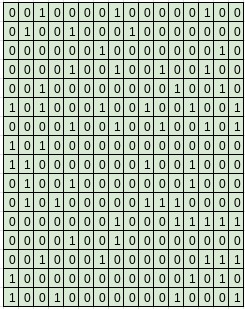
\includegraphics[width=.24\textwidth]{img/ejemploAlgoritmo1.jpeg}
    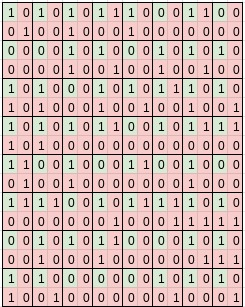
\includegraphics[width=.24\textwidth]{img/ejemploAlgoritmo2.jpeg}
    \caption{Iteraciones con r = 1 (Izquierda) y r = 2 (Derecha)}
    \label{fig:alg1}
\end{figure}

\begin{figure}[H]
    \centering
    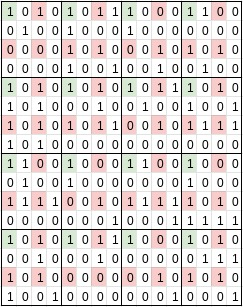
\includegraphics[width=.24\textwidth]{img/ejemploAlgoritmo3.jpeg}
    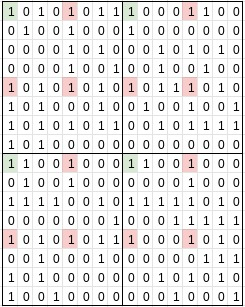
\includegraphics[width=.24\textwidth]{img/ejemploAlgoritmo4.jpeg}
    \caption{Iteraciones con r = 4 (Izquierda) y r = 8 (Derecha)}
    \label{fig:alg2}
\end{figure}

\begin{figure}[H]
    \centering
    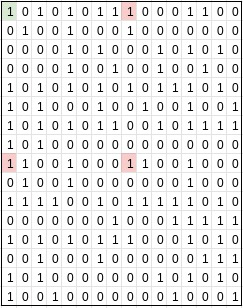
\includegraphics[width=.24\textwidth]{img/ejemploAlgoritmo5.jpeg}
    \caption{Iteracion con r = 16}
    \label{fig:alg3}
\end{figure}


Las casillas señaladas con el color verde corresponden a las casillas que son contadas a la hora de calcular el N (línea 16 en Listado \ref{MatBox2D}). Para el cálculo del valor de las casillas de color verde, se hace una operación OR con los valores calculados en la iteración anterior, es decir la casilla verde y las tres casillas señaladas de color rojo en las Figuras \ref{fig:alg1}, \ref{fig:alg2} y \ref{fig:alg3} (ver líneas 9-15 en Listado \ref{MatBox2D}).


	
	\newpage
	\bibliography{bibliografia}
	\bibliographystyle{apacite}
	
\end{document}

